\chapter{Préliminaires -- Notions de base en électronique}

\section{Savoir lire un schéma électronique}\label{sec:schematic}

Lire un schéma électronique consiste à interpréter un ensemble de symboles normalisés
qui représentent les composants, ainsi que leurs connexions entre eux.
Un schéma ne montre pas l’agencement physique des composants sur une carte, mais leur
relation électrique. Comme le plan du m\'etro, les distances et angles ne sont pas
à l’échelle, mais les connexions sont correctes.

\subsection{Les symboles de base}

Chaque composant est représenté par un symbole normalisé, les symboles seront présentés
au fur et à mesure dans le document.
Voici quelques exemples de symboles courants :
\begin{itemize}
    \item \textbf{Résistance} :
    \raisebox{-0.5\height}{%
        \begin{circuitikz}
            \draw (0,0) to[R] (2,0);
        \end{circuitikz}
    }

    \item \textbf{Condensateur} :
    \raisebox{-0.5\height}{%
        \begin{circuitikz}
            \draw (0,0) to[C] (2,0);
        \end{circuitikz}
    }

    \item \textbf{Diode} :
    \raisebox{-0.5\height}{%
        \begin{circuitikz}
            \draw (0,0) to[D] (2,0);
        \end{circuitikz}
    }

    \item \textbf{Transistor NPN} :
    \raisebox{-0.5\height}{%
        \begin{circuitikz}
            \draw (0,0) to[short, o-o] (2,0);
            \draw (1,0) node[npn, anchor=B, rotate=0]{};
        \end{circuitikz}
    }

    \item \textbf{Source de tension} :
    \raisebox{-0.5\height}{%
        \begin{circuitikz}
            \draw (0,0) to[V] (2,0);
        \end{circuitikz}
    }

    \item \textbf{Source de courant} :
    \raisebox{-0.5\height}{%
        \begin{circuitikz}
            \draw (0,0) to[I] (2,0);
        \end{circuitikz}
    }

    \item \textbf{Masse} :
    \raisebox{-0.5\height}{%
        \begin{circuitikz}
            \draw (0,0) node[ground]{};
        \end{circuitikz}
    }

    \item \textbf{Op-amp} :
    \raisebox{-0.5\height}{%
        \begin{circuitikz}
            \draw (0,0) node[op amp, anchor=-] {};
        \end{circuitikz}
    }

    \item \textbf{Inductance} :
    \raisebox{-0.5\height}{%
        \begin{circuitikz}
            \draw (0,0) to[L] (2,0);
        \end{circuitikz}
    }

    \item \textbf{Interrupteur} :
    \raisebox{-0.5\height}{%
        \begin{circuitikz}
            \draw (0,0) to[spst] (2,0);
        \end{circuitikz}
    }
\end{itemize}

\subsection{Les connexions et nœuds}

Les fils reliant les symboles indiquent les conducteurs électriques.
Un point marqué par un \textbf{nœud} (un petit rond noir) représente une connexion entre plusieurs fils.
En revanche, deux fils qui se croisent sans point ne sont pas connectés.

\begin{figure}[H]
  \centering
  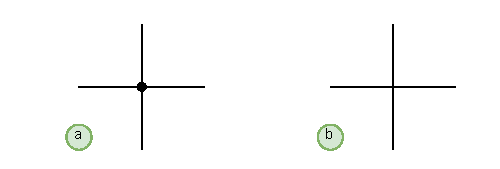
\includegraphics[width=0.8\textwidth]{wires.pdf}
  \caption{\fakecustommacro{a} : fils connectés avec un nœud. \fakecustommacro{b} : fils croisés sans connexion.}
\end{figure}


\subsection{Fl\'echage des tensions et des courants}
Pour analyser un circuit, il est souvent utile de flécher les tensions et les courants.
\begin{itemize}
    \item \textbf{Tension} : La tension est une différence de potentiel entre deux points.
    On flèche la tension de la borne positive (\(+\)) vers la borne négative (\(-\)).
    \item \textbf{Courant} : Le courant est le flux de charges électriques.
    On flèche le courant dans la direction du flux des charges positives (de \(+\) vers \(-\)).
\end{itemize}
Ces flèches aident à visualiser comment l’énergie circule dans le circuit.

\subsection{Exemple simple}

\begin{figure}[H]
    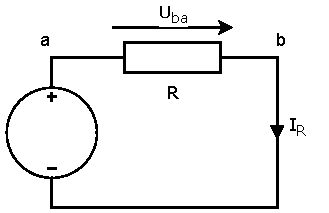
\includegraphics[width=0.7\textwidth]{example-schema.pdf}
    \caption{
        Un schéma de maille simple avec une source de tension et une r\'esistance
    }
\end{figure}

\subsection{La lecture d’un circuit}

\begin{Note}
Pour lire un schéma, on suit généralement ces étapes :
\begin{enumerate}
  \item Identifier la source d’énergie (pile, alimentation).
  \item Repérer la masse (référence commune du circuit), si elle est présente.
  \item Suivre le parcours du courant à travers les composants.
  \item Reconnaître les sous-circuits classiques : diviseur de tension, filtre RC, pont redresseur, etc.
\end{enumerate}

Pour une analyse d'un circuit complexe, on peut ignorer les valeurs des composants et se concentrer sur la topologie du circuit,
c'est-à-dire repérer comment les montages courants comme les redresseurs, amplificateurs, oscillateurs, etc. sont interconnectés.
\end{Note}
